
\subsection{Work Breakdown Structure}


\begin{figure}[h!]
	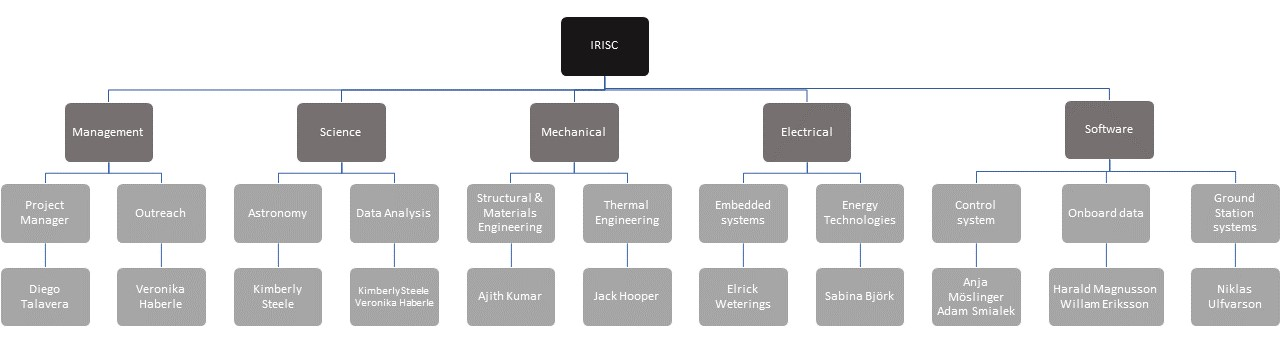
\includegraphics[width=1\textwidth]{3-project-planning/img/WBS_1.jpg}
	\caption{Yes, it looks ugly, I'll change it later, also the WBS below (Diego)}
\end{figure}


\begin{tikzpicture}[scale=\textwidth/18cm,
level 1/.style={sibling distance=40mm},
edge from parent/.style={->,draw},
>=latex]

% root of the the initial tree, level 1
\node[root] {IRISC}
% The first level, as children of the initial tree
child {node[level 2] (c1) {Management}}
child {node[level 2] (c2) {Science}}
child {node[level 2] (c3) {Mechanical}}
child {node[level 2] (c4) {Electrical}}
child {node[level 2] (c5) {Software}};
% The second level, relatively positioned nodes

\begin{scope}[every node/.style={level 3}]
\node [below of = c1, xshift=15pt] (c11) {Setting shape};
\node [below of = c11] (c12) {Choosing color};
\node [below of = c12] (c13) {Adding shading};

\node [below of = c2, xshift=15pt] (c21) {Using a Matrix};
\node [below of = c21] (c22) {Relatively};
\node [below of = c22] (c23) {Absolutely};
\node [below of = c23] (c24) {Using overlays};

\node [below of = c3, xshift=15pt] (c31) {Default arrows};
\node [below of = c31] (c32) {Arrow library};
\node [below of = c32] (c33) {Resizing tips};
\node [below of = c33] (c34) {Shortening};
\node [below of = c34] (c35) {Bending};
\end{scope}

% lines from each level 1 node to every one of its "children"
\foreach \value in {1,2,3}
\draw[->] (c1.195) |- (c1\value.west);

\foreach \value in {1,...,4}
\draw[->] (c2.195) |- (c2\value.west);

\foreach \value in {1,...,5}
\draw[->] (c3.195) |- (c3\value.west);
\end{tikzpicture}